\documentclass{article}
\usepackage[utf8]{inputenc}
\usepackage{algorithm}
\usepackage{algpseudocode}
\usepackage{tikz}
\usetikzlibrary{automata,topaths}
\usepackage{pgfplots, pgfplotstable}
\usepackage{listings} 
\lstset{language=Python}

\title{MC886 - Machine learning \\ Exercise 1}
\author{Rafael Almeida Erthal Hermano\\RA 121286}
\date{March 2014}

\begin{document}

\maketitle
\newpage

\section{The data}

The data consists of 151 records with 4 float attributes A,B,C,D.

\begin{table}[h]
    \begin{tabular}{|l|l|l|l|l}
        \cline{1-4}
        \textbf{Attribute A} & \textbf{Attribute B} & \textbf{Attribute C} & \textbf{Attribute D} &  \\ \cline{1-4}
        5.1 & 3.5 & 1.4 & 0.2 \\ \cline{1-4}
        4.9 & 3   & 1.4 & 0.2 \\ \cline{1-4}
        4.7 & 3.2 & 1.3 & 0.2 \\ \cline{1-4}
        4.6 & 3.1 & 1.5 & 0.2 \\ \cline{1-4}
        5   & 3.6 & 1.4 & 0.2 \\ \cline{1-4}
    \end{tabular}
\end{table}

To read the data the following function was implemented

\begin{lstlisting}
def read_data:
    import sys
    file = []
    for line in sys.stdin:
        file.append(line)
        
    return [[float(d) for d in r[0:-1].split('\t')] for r in file[1:]]
\end{lstlisting}

\subsection{Wrong records}
The records in line 36 and 50 where removed because they where with missing data, and the record in line 59 where removed because its a invalid number.

\begin{table}[h]
    \begin{tabular}{|l|l|l|l|l}
        \cline{1-4}
        \textbf{Attribute A} & \textbf{Attribute B} & \textbf{Attribute C} & \textbf{Attribute D} &  \\ \cline{1-4}
        4.9 & 3.1 & & 0.2 \\ \cline{1-4}
        5.3 & & 1.5 & 0.2 \\ \cline{1-4}
        4.9 & 2.4 & 12.4.3 & 1 \\ \cline{1-4}
    \end{tabular}
\end{table}

\newpage
\subsection{Histograms}
For each data attribute two histograms where built, one with 10 bins and another with 30 bins.

\begin{table}[h]
\begin{tabular}{cl}
    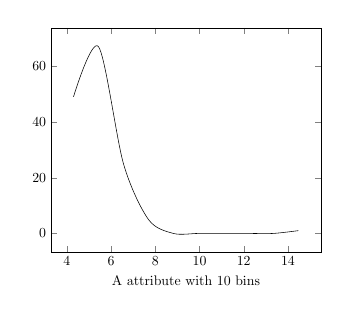
\begin{tikzpicture}[scale=0.5]
      \begin{axis}[xlabel=A attribute with 10 bins]
        \addplot[smooth] coordinates {( 4.30 , 49.00 ) ( 5.43 , 67.00 ) ( 6.56 , 25.00 ) ( 7.69 , 5.00 ) ( 8.82 , 0.00 ) ( 9.95 , 0.00 ) ( 11.08 , 0.00 ) ( 12.21 , 0.00 ) ( 13.34 , 0.00 ) ( 14.47 , 1.00 )};
      \end{axis}
    \end{tikzpicture}
 & 
    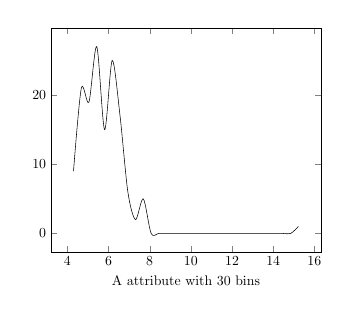
\begin{tikzpicture}[scale=0.5]
      \begin{axis}[xlabel=A attribute with 30 bins]
        \addplot[smooth] coordinates {( 4.30 , 9.00 ) ( 4.68 , 21.00 ) ( 5.05 , 19.00 ) ( 5.43 , 27.00 ) ( 5.81 , 15.00 ) ( 6.18 , 25.00 ) ( 6.56 , 17.00 ) ( 6.94 , 6.00 ) ( 7.31 , 2.00 ) ( 7.69 , 5.00 ) ( 8.07 , 0.00 ) ( 8.44 , 0.00 ) ( 8.82 , 0.00 ) ( 9.20 , 0.00 ) ( 9.57 , 0.00 ) ( 9.95 , 0.00 ) ( 10.33 , 0.00 ) ( 10.70 , 0.00 ) ( 11.08 , 0.00 ) ( 11.46 , 0.00 ) ( 11.83 , 0.00 ) ( 12.21 , 0.00 ) ( 12.59 , 0.00 ) ( 12.96 , 0.00 ) ( 13.34 , 0.00 ) ( 13.72 , 0.00 ) ( 14.09 , 0.00 ) ( 14.47 , 0.00 ) ( 14.85 , 0.00 ) ( 15.22 , 1.00 )};
      \end{axis}
    \end{tikzpicture}
    \\
    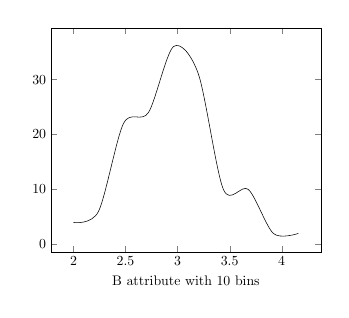
\begin{tikzpicture}[scale=0.5]
      \begin{axis}[xlabel=B attribute with 10 bins]
        \addplot[smooth] coordinates {( 2.00 , 4.00 ) ( 2.24 , 6.00 ) ( 2.48 , 22.00 ) ( 2.72 , 24.00 ) ( 2.96 , 36.00 ) ( 3.20 , 31.00 ) ( 3.44 , 10.00 ) ( 3.68 , 10.00 ) ( 3.92 , 2.00 ) ( 4.16 , 2.00 )};
      \end{axis}
    \end{tikzpicture}
 & 
    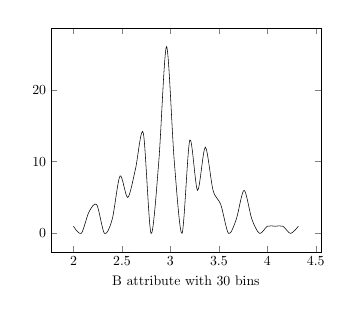
\begin{tikzpicture}[scale=0.5]
      \begin{axis}[xlabel=B attribute with 30 bins]
        \addplot[smooth] coordinates {( 2.00 , 1.00 ) ( 2.08 , 0.00 ) ( 2.16 , 3.00 ) ( 2.24 , 4.00 ) ( 2.32 , 0.00 ) ( 2.40 , 2.00 ) ( 2.48 , 8.00 ) ( 2.56 , 5.00 ) ( 2.64 , 9.00 ) ( 2.72 , 14.00 ) ( 2.80 , 0.00 ) ( 2.88 , 10.00 ) ( 2.96 , 26.00 ) ( 3.04 , 10.00 ) ( 3.12 , 0.00 ) ( 3.20 , 13.00 ) ( 3.28 , 6.00 ) ( 3.36 , 12.00 ) ( 3.44 , 6.00 ) ( 3.52 , 4.00 ) ( 3.60 , 0.00 ) ( 3.68 , 2.00 ) ( 3.76 , 6.00 ) ( 3.84 , 2.00 ) ( 3.92 , 0.00 ) ( 4.00 , 1.00 ) ( 4.08 , 1.00 ) ( 4.16 , 1.00 ) ( 4.24 , 0.00 ) ( 4.32 , 1.00 )};
      \end{axis}
    \end{tikzpicture}
    \\
    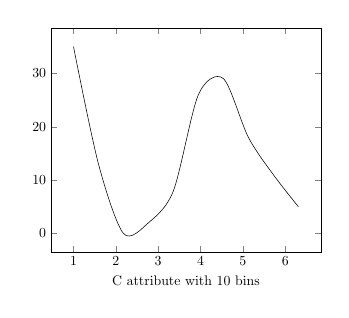
\begin{tikzpicture}[scale=0.5]
      \begin{axis}[xlabel=C attribute with 10 bins]
        \addplot[smooth] coordinates {( 1.00 , 35.00 ) ( 1.59 , 13.00 ) ( 2.18 , 0.00 ) ( 2.77 , 2.00 ) ( 3.36 , 8.00 ) ( 3.95 , 26.00 ) ( 4.54 , 29.00 ) ( 5.13 , 18.00 ) ( 5.72 , 11.00 ) ( 6.31 , 5.00 )};
      \end{axis}
    \end{tikzpicture}
 & 
    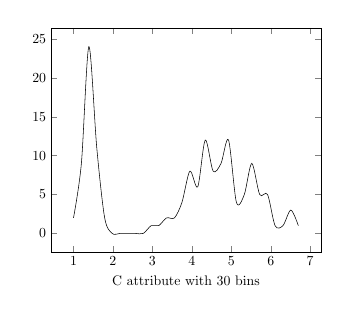
\begin{tikzpicture}[scale=0.5]
      \begin{axis}[xlabel=C attribute with 30 bins]
        \addplot[smooth] coordinates {( 1.00 , 2.00 ) ( 1.20 , 9.00 ) ( 1.39 , 24.00 ) ( 1.59 , 11.00 ) ( 1.79 , 2.00 ) ( 1.98 , 0.00 ) ( 2.18 , 0.00 ) ( 2.38 , 0.00 ) ( 2.57 , 0.00 ) ( 2.77 , 0.00 ) ( 2.97 , 1.00 ) ( 3.16 , 1.00 ) ( 3.36 , 2.00 ) ( 3.56 , 2.00 ) ( 3.75 , 4.00 ) ( 3.95 , 8.00 ) ( 4.15 , 6.00 ) ( 4.34 , 12.00 ) ( 4.54 , 8.00 ) ( 4.74 , 9.00 ) ( 4.93 , 12.00 ) ( 5.13 , 4.00 ) ( 5.33 , 5.00 ) ( 5.52 , 9.00 ) ( 5.72 , 5.00 ) ( 5.92 , 5.00 ) ( 6.11 , 1.00 ) ( 6.31 , 1.00 ) ( 6.51 , 3.00 ) ( 6.70 , 1.00 )};
      \end{axis}
    \end{tikzpicture}
    \\
    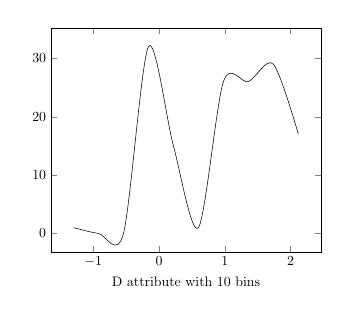
\begin{tikzpicture}[scale=0.5]
      \begin{axis}[xlabel=D attribute with 10 bins]
        \addplot[smooth] coordinates {( -1.30 , 1.00 ) ( -0.92 , 0.00 ) ( -0.54 , 0.00 ) ( -0.16 , 32.00 ) ( 0.22 , 15.00 ) ( 0.60 , 1.00 ) ( 0.98 , 26.00 ) ( 1.36 , 26.00 ) ( 1.74 , 29.00 ) ( 2.12 , 17.00 )};
      \end{axis}
    \end{tikzpicture}
 & 
    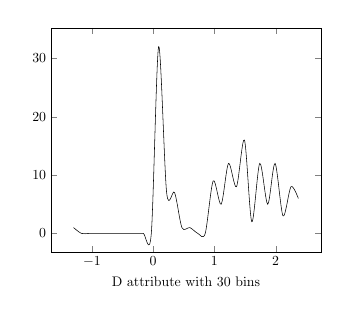
\begin{tikzpicture}[scale=0.5]
      \begin{axis}[xlabel=D attribute with 30 bins]
        \addplot[smooth] coordinates {( -1.30 , 1.00 ) ( -1.17 , 0.00 ) ( -1.05 , 0.00 ) ( -0.92 , 0.00 ) ( -0.79 , 0.00 ) ( -0.67 , 0.00 ) ( -0.54 , 0.00 ) ( -0.41 , 0.00 ) ( -0.29 , 0.00 ) ( -0.16 , 0.00 ) ( -0.03 , 0.00 ) ( 0.09 , 32.00 ) ( 0.22 , 7.00 ) ( 0.35 , 7.00 ) ( 0.47 , 1.00 ) ( 0.60 , 1.00 ) ( 0.73 , 0.00 ) ( 0.85 , 0.00 ) ( 0.98 , 9.00 ) ( 1.11 , 5.00 ) ( 1.23 , 12.00 ) ( 1.36 , 8.00 ) ( 1.49 , 16.00 ) ( 1.61 , 2.00 ) ( 1.74 , 12.00 ) ( 1.87 , 5.00 ) ( 1.99 , 12.00 ) ( 2.12 , 3.00 ) ( 2.25 , 8.00 ) ( 2.37 , 6.00 )};
      \end{axis}
    \end{tikzpicture}
\end{tabular}
\end{table}

\subsection{Outliers}
From the attrubute A histogram we can see that only one value is very diferente from the others, while all values are bellow 8.82, one record has the value 15.6, so this value will be removed from the data, because it is an outlier.
\newpage

\subsection{Covariance matrix}
Covariance is a measure of how much two variables change together.  The sign of the covariance shows the tendency in the linear relationship between two variablesand the normalized version of the covariance, the correlation coefficient shows by its magnitude the strength of the linear relation. The covariance of two varibles can be defined as:

\begin{equation}
    g(x,y) = E[(x - E(x)) \cdot (y - E(y))]
    \label{eq:conv_eq}
\end{equation}

Where $E[x]$ is the expected value for x, and can be defined as:

\begin{equation}
    E[X] = \sum_{i = 1}^{k} x_{i} \cdot p_{i}
    \label{eq:expec_val}
\end{equation}

Where $k$ is the number os elements in the vector and $p_{i}$ is the probability of the element $x_{i}$.

The covariance matrix is a matrix where the elements $x[i][j]$ represents the covariance betwen the attribute $i$  with the element $j$.

\begin{lstlisting}[frame=single]
import numpy as np

print np.cov(read_data(), rowvar=None)
\end{lstlisting}

The computed covariance matrix for the data withou the outliers is:
\begin{table}[h]
    \begin{tabular}{|l|l|l|l|l|l}
        \hline
        & \textbf{A} & \textbf{B} & \textbf{C} & \textbf{D}  \\ \hline
        \textbf{A} & 0.68955314  & -0.04529523  & 1.28332735  & 0.52535853   \\ \hline
        \textbf{B} & -0.04529523 &  0.18935664  & -0.33002551 & -0.11114124  \\ \hline
        \textbf{C} & 1.28332735  & -0.33002551  & 3.12865234  & 1.2951299    \\ \hline
        \textbf{D} & 0.52535853  & -0.11114124  & 1.2951299   & 0.62591403   \\ \hline
    \end{tabular}
\end{table}
\newpage

\subsection{PCA}
Principal component analysis is a procedure that uses orthogonal transformation to convert a set of variables into a set of values of linearly uncorrelated variables called principal components. The number of principal components is less than or equal to the number of original variables.

\begin{lstlisting}[frame=single]
from sklearn.decomposition import PCA

pca = PCA(n_components=2)
pca.fit(read_data())
print pca.explained_variance_ratio_
\end{lstlisting}

The computed values for PCA are:
\begin{table}[h]
    \begin{tabular}{|l|l|l|l|l}
        \hline
        0.91742359 &  0.05143194 &  0.02201535 & 0.00912912 \\ \hline
    \end{tabular}
\end{table}

\subsubsection{Ploting data}

The first and second component are much bigger than the others, so we should keep only two dimensions.


\begin{lstlisting}[frame=single]
from sklearn.decomposition import PCA

pca = PCA(n_components=2)
print pca.fit_transform(read_data())
\end{lstlisting}

\begin{center}
\begin{tikzpicture}
\draw[<->] (-3,0)--(3,0);
\draw[<->] (0,-2)--(0,2);
\draw ( -2.71614909084 , -0.316485390033 ) node[anchor=south] {.};
\draw ( -2.74693928225 , 0.182813855105 ) node[anchor=south] {.};
\draw ( -2.92164943268 , 0.144210519862 ) node[anchor=south] {.};
\draw ( -2.77849391742 , 0.320662772551 ) node[anchor=south] {.};
\draw ( -2.76073854621 , -0.326287951802 ) node[anchor=south] {.};
\draw ( -2.31203979918 , -0.744082537689 ) node[anchor=south] {.};
\draw ( -2.85298093106 , 0.0817294245717 ) node[anchor=south] {.};
\draw ( -2.65852481528 , -0.159031349048 ) node[anchor=south] {.};
\draw ( -2.91983908537 , 0.578576219409 ) node[anchor=south] {.};
\draw ( -2.70581725108 , 0.125230420984 ) node[anchor=south] {.};
\draw ( -2.53855571314 , -0.638725470647 ) node[anchor=south] {.};
\draw ( -2.64548999508 , -0.0113798698319 ) node[anchor=south] {.};
\draw ( -2.8192554549 , 0.244688038561 ) node[anchor=south] {.};
\draw ( -3.25709022273 , 0.509326572227 ) node[anchor=south] {.};
\draw ( -2.67518033008 , -1.17541422736 ) node[anchor=south] {.};
\draw ( -2.41606387741 , -1.34570483999 ) node[anchor=south] {.};
\draw ( -2.65416475795 , -0.820075384505 ) node[anchor=south] {.};
\draw ( -2.68008112794 , -0.314032939733 ) node[anchor=south] {.};
\draw ( -2.23102188722 , -0.865385693731 ) node[anchor=south] {.};
\draw ( -2.6195736251 , -0.517422314604 ) node[anchor=south] {.};
\draw ( -2.3424694969 , -0.378341460663 ) node[anchor=south] {.};
\draw ( -2.57516441658 , -0.440840668779 ) node[anchor=south] {.};
\draw ( -3.24785634398 , -0.144974263595 ) node[anchor=south] {.};
\draw ( -2.33466899181 , -0.10387501297 ) node[anchor=south] {.};
\draw ( -2.388896276 , 0.0456147652803 ) node[anchor=south] {.};
\draw ( -2.53962859311 , 0.156483644757 ) node[anchor=south] {.};
\draw ( -2.50085764978 , -0.135128236743 ) node[anchor=south] {.};
\draw ( -2.5943696414 , -0.361813812085 ) node[anchor=south] {.};
\draw ( -2.67155963548 , -0.306682828263 ) node[anchor=south] {.};
\draw ( -2.66505571359 , 0.201205154974 ) node[anchor=south] {.};
\draw ( -2.62046625823 , 0.211007716744 ) node[anchor=south] {.};
\draw ( -2.44139605048 , -0.411432983471 ) node[anchor=south] {.};
\draw ( -2.68048507801 , -0.809041435536 ) node[anchor=south] {.};
\draw ( -2.62954497117 , -1.09269629373 ) node[anchor=south] {.};
\draw ( -2.89843604312 , -0.0677675931095 ) node[anchor=south] {.};
\draw ( -2.65668749154 , -0.59279013676 ) node[anchor=south] {.};
\draw ( -2.83305471886 , -0.264413768347 ) node[anchor=south] {.};
\draw ( -3.01371157069 , 0.48544881218 ) node[anchor=south] {.};
\draw ( -2.62227660553 , -0.223357982803 ) node[anchor=south] {.};
\draw ( -2.80186057738 , -0.268704517681 ) node[anchor=south] {.};
\draw ( -2.88300667871 , 0.942478997401 ) node[anchor=south] {.};
\draw ( -3.03039406192 , 0.33719042113 ) node[anchor=south] {.};
\draw ( -2.43706296959 , -0.204352531668 ) node[anchor=south] {.};
\draw ( -2.24138070342 , -0.438977017488 ) node[anchor=south] {.};
\draw ( -2.74711952909 , 0.249592939161 ) node[anchor=south] {.};
\draw ( -2.57011034831 , -0.5008765532 ) node[anchor=south] {.};
\draw ( -2.87236640273 , 0.227535365322 ) node[anchor=south] {.};
\draw ( -2.73571480935 , -0.103900365227 ) node[anchor=south] {.};
\draw ( 1.25293709597 , -0.659933454981 ) node[anchor=south] {.};
\draw ( 0.900453320996 , -0.309517625554 ) node[anchor=south] {.};
\draw ( 1.43216057413 , -0.481028751992 ) node[anchor=south] {.};
\draw ( 0.149498519545 , 0.836688878854 ) node[anchor=south] {.};
\draw ( 1.05559775291 , -0.0583292655051 ) node[anchor=south] {.};
\draw ( 0.607944909421 , 0.432380692237 ) node[anchor=south] {.};
\draw ( 1.06299430792 , -0.278871313615 ) node[anchor=south] {.};
\draw ( 1.01136879123 , -0.201689995386 ) node[anchor=south] {.};
\draw ( -0.0420743689626 , 0.716606236617 ) node[anchor=south] {.};
\draw ( -0.542578879524 , 1.27836122479 ) node[anchor=south] {.};
\draw ( 0.479301044408 , 0.103379299163 ) node[anchor=south] {.};
\draw ( 0.230876925194 , 0.5818275547 ) node[anchor=south] {.};
\draw ( 0.951726945088 , 0.141393835397 ) node[anchor=south] {.};
\draw ( -0.206425703189 , 0.251594225131 ) node[anchor=south] {.};
\draw ( 0.895939993262 , -0.449818993301 ) node[anchor=south] {.};
\draw ( 0.627150134244 , 0.353353835543 ) node[anchor=south] {.};
\draw ( 0.202205517301 , 0.35883305629 ) node[anchor=south] {.};
\draw ( 0.911369357678 , 0.56042759721 ) node[anchor=south] {.};
\draw ( 0.0113970725563 , 0.600200741744 ) node[anchor=south] {.};
\draw ( 1.08400988005 , 0.0764675292376 ) node[anchor=south] {.};
\draw ( 0.325281549946 , 0.0800830986934 ) node[anchor=south] {.};
\draw ( 1.26471878935 , 0.349706223694 ) node[anchor=south] {.};
\draw ( 0.887932264899 , 0.210618130322 ) node[anchor=south] {.};
\draw ( 0.682278652655 , -0.130031362987 ) node[anchor=south] {.};
\draw ( 0.868033029132 , -0.31136316402 ) node[anchor=south] {.};
\draw ( 1.29933689864 , -0.215765193665 ) node[anchor=south] {.};
\draw ( 1.52567256575 , -0.254343176651 ) node[anchor=south] {.};
\draw ( 0.780484218856 , 0.170176496045 ) node[anchor=south] {.};
\draw ( -0.338888884992 , 0.383299615346 ) node[anchor=south] {.};
\draw ( -0.102041131268 , 0.719658359321 ) node[anchor=south] {.};
\draw ( -0.223640333865 , 0.698207697316 ) node[anchor=south] {.};
\draw ( 0.103278963721 , 0.325741533482 ) node[anchor=south] {.};
\draw ( 1.34642211116 , 0.43487660762 ) node[anchor=south] {.};
\draw ( 0.554653714747 , 0.482007103054 ) node[anchor=south] {.};
\draw ( 0.77484595367 , -0.198017031281 ) node[anchor=south] {.};
\draw ( 1.18860167525 , -0.390371907888 ) node[anchor=south] {.};
\draw ( 0.781609156308 , 0.398068655624 ) node[anchor=south] {.};
\draw ( -0.804951007187 , 0.62466678 ) node[anchor=south] {.};
\draw ( 0.430531778562 , 0.687841688795 ) node[anchor=south] {.};
\draw ( 0.857854459777 , 0.0482664281676 ) node[anchor=south] {.};
\draw ( 0.197151449033 , 0.418868940711 ) node[anchor=south] {.};
\draw ( -0.738665095765 , 1.0179772148 ) node[anchor=south] {.};
\draw ( 0.323444226209 , 0.513841886406 ) node[anchor=south] {.};
\draw ( 0.2986007362 , 0.224675215774 ) node[anchor=south] {.};
\draw ( 0.343009944722 , 0.3012568616 ) node[anchor=south] {.};
\draw ( 0.609782233158 , -0.00137809547541 ) node[anchor=south] {.};
\draw ( -0.93962513343 , 0.750850005186 ) node[anchor=south] {.};
\draw ( 0.265819950646 , 0.356387845421 ) node[anchor=south] {.};
\draw ( 2.49951209007 , -0.00982250876085 ) node[anchor=south] {.};
\draw ( 1.38212958037 , 0.570887226032 ) node[anchor=south] {.};
\draw ( 2.58471841361 , -0.330856005136 ) node[anchor=south] {.};
\draw ( 1.93827637344 , 0.193534274423 ) node[anchor=south] {.};
\draw ( 2.31776587832 , 0.0385580359945 ) node[anchor=south] {.};
\draw ( 3.3646781402 , -0.519501691987 ) node[anchor=south] {.};
\draw ( 0.487254819901 , 1.17919115006 ) node[anchor=south] {.};
\draw ( 2.89947714878 , -0.316744581207 ) node[anchor=south] {.};
\draw ( 2.2876966743 , 0.270740944908 ) node[anchor=south] {.};
\draw ( 2.88625348065 , -0.792151587435 ) node[anchor=south] {.};
\draw ( 1.63022878343 , -0.247592737585 ) node[anchor=south] {.};
\draw ( 1.77068131825 , 0.222923846905 ) node[anchor=south] {.};
\draw ( 2.13384882559 , -0.213868950685 ) node[anchor=south] {.};
\draw ( 1.31310058507 , 0.766926489434 ) node[anchor=south] {.};
\draw ( 1.55412814927 , 0.509020282007 ) node[anchor=south] {.};
\draw ( 1.87324694178 , -0.13791232952 ) node[anchor=south] {.};
\draw ( 1.91690030763 , -0.0282464003183 ) node[anchor=south] {.};
\draw ( 3.45579558761 , -1.15541122794 ) node[anchor=south] {.};
\draw ( 3.76302097731 , -0.225412007929 ) node[anchor=south] {.};
\draw ( 1.26652913665 , 0.784071923242 ) node[anchor=south] {.};
\draw ( 2.39661294929 , -0.383552651483 ) node[anchor=south] {.};
\draw ( 1.16629739877 , 0.58986732491 ) node[anchor=south] {.};
\draw ( 3.46707211798 , -0.419024173288 ) node[anchor=south] {.};
\draw ( 1.35624018682 , 0.208805183544 ) node[anchor=south] {.};
\draw ( 2.24363935837 , -0.333933480097 ) node[anchor=south] {.};
\draw ( 2.5816114831 , -0.531800169139 ) node[anchor=south] {.};
\draw ( 1.22611949176 , 0.180004410071 ) node[anchor=south] {.};
\draw ( 1.25872003047 , 0.11507086448 ) node[anchor=south] {.};
\draw ( 2.09106971752 , 0.210694187092 ) node[anchor=south] {.};
\draw ( 2.35509556914 , -0.426443102097 ) node[anchor=south] {.};
\draw ( 2.80907208767 , -0.342485992546 ) node[anchor=south] {.};
\draw ( 3.19956236222 , -1.34596403116 ) node[anchor=south] {.};
\draw ( 2.12713768042 , 0.213146637393 ) node[anchor=south] {.};
\draw ( 1.41075753188 , 0.165315060527 ) node[anchor=south] {.};
\draw ( 1.74653183919 , 0.534765327309 ) node[anchor=south] {.};
\draw ( 3.04540607729 , -0.673914483663 ) node[anchor=south] {.};
\draw ( 2.11297792278 , -0.162397001403 ) node[anchor=south] {.};
\draw ( 1.87231085226 , -0.0380489620877 ) node[anchor=south] {.};
\draw ( 1.13694058103 , 0.160399286532 ) node[anchor=south] {.};
\draw ( 2.07622455002 , -0.37132299167 ) node[anchor=south] {.};
\draw ( 2.28299449862 , -0.19731594985 ) node[anchor=south] {.};
\draw ( 1.89176675675 , -0.423412726182 ) node[anchor=south] {.};
\draw ( 1.38212958037 , 0.570887226032 ) node[anchor=south] {.};
\draw ( 2.53142721893 , -0.281229594319 ) node[anchor=south] {.};
\draw ( 2.38791120999 , -0.324123678896 ) node[anchor=south] {.};
\draw ( 1.91314282256 , -0.201632051441 ) node[anchor=south] {.};
\draw ( 1.49452188066 , 0.378514236599 ) node[anchor=south] {.};
\draw ( 1.73244251436 , -0.0803361348303 ) node[anchor=south] {.};
\draw ( 1.86959927074 , -0.138519241355 ) node[anchor=south] {.};
\draw ( 1.35728609036 , 0.2817205554 ) node[anchor=south] {.};
\end{tikzpicture}
\end{center}

\end{document}
